\documentclass{article}
\usepackage[utf8]{inputenc}
\usepackage{hyperref}
\usepackage{graphicx}

\title{Organiz-Asso}
\author{Axel CERESA - 21103270 \\ Daba KONE -}
\date{}

\begin{document}

\maketitle

\newpage

\section{Rapport}

\subsection{Répartition du travail}
Notre binôme est un petit peu particulier. Daba était dans un autre groupe puis dans une autre classe avant de me rejoindre (Axel). A ce moment, une grande partie du travail avait déjà été réalisée.\\

- Axel : Tout le backend et le frontend.

- Daba : Tests Postman de toutes les requêtes.

\subsection{Difficultés}
La principale difficulté que nous avons rencontrée concerne l'utilisation de express-session pour générer la connexion et la déconnexion d'un utilisateur. L'utilisation des cookies de session n'était pas évidente à comprendre au départ.

L'autre difficulté était de comprendre comment bien utiliser les requêtes \texttt{axios} et les \texttt{useEffect} pour actualiser en permanence les messages des forums et que la page reste à jour sans avoir besoin de recharger la page.

\subsection{Fonctionnalités}
L'ensemble des fonctionnalités demandées dans le cahier des charges ont été réalisées et d'autres supplémentaires ont été ajoutées, notamment :

\begin{enumerate}
    \item La possibilité de créer/supprimer un forum et de modifier son nom et ses restrictions.
    \item La possibilité de modifier un message.
    \item Options de modérations pour les administrateurs qui peuvent supprimer n'importe quel message posté sur le site.
\end{enumerate}

Si nous avions eu le temps, nous aurions aimé implémenter d'autres fonctionnalités tels que l'ajout d'une photo de profil, la possibilité créer une biographie pour son profil ou même la possibilité de like des messages et de les ajouter en favoris.
De plus, l'ajout d'un genre de calendrier / liste d'évènements (création et suppression) aurait pu être intéressant.

\subsection{Choix d'implémentation}
Concernant les choix d'implémentation, nous avons utilisé \texttt{react-router-dom} pour gérer les routes et les urls du site côté client.

Pour la base de données, notre choix de créer une collection différente pour les commentaires au lieu de les intégrer directement dans la description d'un message n'est peut-être pas la meilleur solution car cela multiplie le nombre de requête au serveur, ce qui n'est pas très efficace.

\begin{figure}
    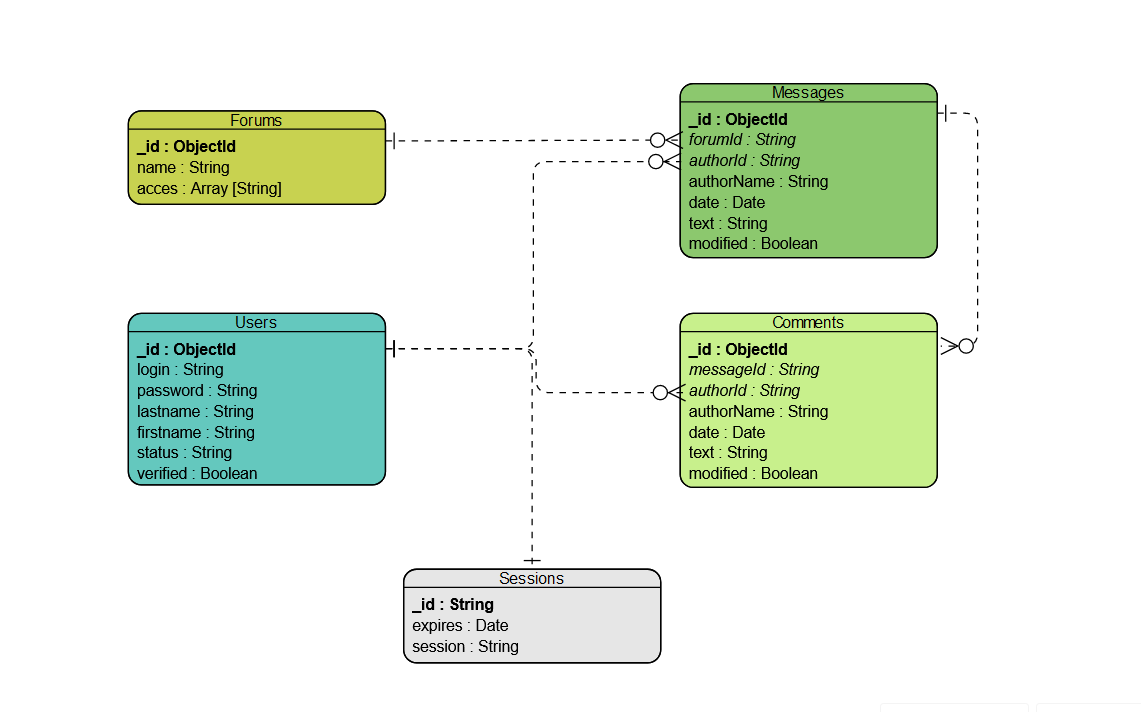
\includegraphics[width=1\textwidth]{BDD.png}
    \caption{Base de données}
    \includegraphics[width=1\textwidth]{archi_react.png}
    \caption{Architecture des composants react}
\end{figure}

\newpage

\section{Installation}
Une fois les fichiers téléchargés, dans un terminal faire un \texttt{npm install} dans le répertoire \texttt{/server} et dans le répertoire \texttt{/client} pour installer les dépendances nécessaires.

Pour relier la base de données au backend, modifier côté serveur dans le fichier \texttt{/config/db.js} la ligne 2 \texttt{const url = "url\_mongodb";} par le lien de votre base de données MongoDB. Créer une base de données Organiz-Asso et y importer les collections sous format .json présentes dans le répertoire \texttt{Collections}.

\section{BACKEND}

\subsection*{Architecture des fichiers}
Dans le dossier \texttt{/server} se trouve tous les fichiers réalisant le backend de notre application dont le point d'entrée est \texttt{index.js}. Ensuite, \texttt{app.js} lance le server et fait appel à \texttt{api.js} qui gère toutes les routes de notre backend.

\begin{enumerate}
    \item \texttt{/config} : Contient le fichier \texttt{db.js} qui définit les fonctions utilisées dans notre application pour se connecter et se déconnecter de la base de données. Elles sont appelées dans le fichier \texttt{db.middleware.js}.
    \item \texttt{/controllers} : Contient les fichiers définissant toutes les actions possibles sur notre base de données. Elles sont appelées en callback des différentes routes de notre application. Chaque fichier correspond aux fonctions liées à une entité spécifique. Ces fonctions font appel aux méthodes des classes définies dans les fichiers de \texttt{/entities}.
    \item \texttt{/entities} : Contient les fichiers définissant les classes de chaque entités de notre application (user, forum, message, comment). Les méthodes définies dans ces classes effectuent les requêtes auprès de la base de données MongoDB passée en paramètres.
    \item \texttt{/middleware} : Contient les middlewares \texttt{checkUser} et \texttt{requireAuth} utilisés à la racine de notre serveur pour sécuriser les requêtes et restreindre leur accès uniquement à un utilisateur connecté (dont une session express a été créée). A chaque requête, les middlewares \texttt{connectDBMiddleware} et \texttt{closeDBMiddleware} sont appelés.
    \item \texttt{/routes} : Contient les fichiers définissant les routes des requêtes serveur de notre application pour chaque famille de services.
\end{enumerate}

\newpage

\section{FRONTEND}

\subsection*{Architecture des fichiers}
Dans le dossier \texttt{/client} se trouve tous les fichiers réalisant le frontend de notre application. Le point d'entrée est \texttt{index.js}, qui fait appel au composant \texttt{<App/>} qui gère le routage de notre application avec \texttt{react-router-dom}.

\begin{enumerate}
    \item \texttt{/public} : Contient le fichier \texttt{index.html} dans lequel est généré le render des composants react de l'application.
    \item \texttt{/assets/img} : Contient les images/logo temporairement utilisés dans l'application.
    \item \texttt{/components} : Contient les fichiers définissant les différents composants appelés dans les pages de notre application react. Ces composants disposent chacun de leur fichier CSS correspondant. \texttt{AppContext.js} est le composant englobant toute notre application et permet de stocker dans une variable accessible dans tout nos composants les informations de session de l'utilisateur connecté.
    \item \texttt{/pages} : Contient les fichiers définissant les pages de l'application, chacune d'elles fait appel aux composants définis dans le répertoire \texttt{/components}.
\end{enumerate}

\section{BASE DE DONNÉES}
La base de données est définie grâce à MongoDB.

\subsection*{Définition des collections}
Les champs \_id de type \texttt{ObjectId} sont générés automatiquement lors de l'ajout d'un document dans la base de données.

\subsubsection*{users}
\begin{verbatim}
{
   "_id" : ObjectId(),
   "login" : String,
   "password" : String,
   "lastname" : String,
   "firsname" : String,
   "status" : String,
   "date" : Date(),
   "verified" : Boolean
}
\end{verbatim}
Le password est crypté à l'aide de la bibliothèque \texttt{bcrypt} avant l'ajout dans la base de données. Le status d'un user est initialisé de base à "member".

\newpage

\subsubsection*{forums}
\begin{verbatim}
{
   "_id" : ObjectId(),
   "name" : String,
   "acces" : [ String ]
}
\end{verbatim}
Le champs acces définit les status de user pouvant voir et écrire dans le forum.

\subsubsection*{messages}
\begin{verbatim}
{
   "_id" : ObjectId(),
   "forumId" : String,
   "userId" : String,
   "userName" : String,
   "date" : Date(),
   "text" : String,
   "modified" : Boolean
}
\end{verbatim}

\subsubsection*{comments}
\begin{verbatim}
{
   "_id" : ObjectId(),
   "messageId" : String,
   "authorId" : String,
   "authorName" : String,
   "date" : Date(),
   "text" : String,
   "modified" : Boolean
}
\end{verbatim}

\subsubsection*{sessions}
\begin{verbatim}
{
   "_id" : String,
   "expires" : Date(),
   "session" : String
}
\end{verbatim}
Les documents de la collection sessions sont générés automatiquement par express-session et contiennent l'id de la session ainsi que le cookie associé.

\section{Lancement}
Pour lancer le serveur, se placer dans le dossier \texttt{/server} et exécuter la commande \texttt{npm start} dans un terminal. Cela lancera le serveur à l'adresse \url{http://localhost:4000} par défaut.

Pour lancer le client, se placer dans le dossier \texttt{/client} et exécuter la commande \texttt{npm start} dans un terminal. Cela compilera et lancera le client à l'adresse \url{http://localhost:3000} par défaut (le navigateur s'ouvre automatiquement).

\end{document}
